\documentclass[a4paper,11pt]{article}
\pdfoutput=1 % if your are submitting a pdflatex (i.e. if you have
             % images in pdf, png or jpg format)

\usepackage{jinstpub} % for details on the use of the package, please
                     % see the JINST-author-manual

\usepackage{heppennames2}
\usepackage{hepnicenames}

\usepackage[caption=false]{subfig}

\usepackage{feynmp-auto}

\unitlength = 1mm

\makeatletter
\def\endfmffile{%
  \fmfcmd{\p@rcent\space the end.^^J%
          end.^^J%
          endinput;}%
  \if@fmfio
    \immediate\closeout\@outfmf
  \fi
  \ifnum\pdfshellescape=\@ne
    \immediate\write18{mpost \thefmffile}%
  \fi}
\makeatother

\newcommand{\pt}{\ensuremath{p_{\mathrm T}}}

\newcommand{\mh}{\ensuremath{m_{H}} } 
\newcommand{\ptmiss}{\ensuremath{p_{\mathrm T}^{\mathrm{miss}}}}
\newcommand{\chisquare}{\ensuremath{\chi^2}}



\title{\boldmath Reconstruction and classification of tau lepton decays with future \Pelectron\APelectron linear collider}


%% %simple case: 2 authors, same institution
%% \author{A. Uthor}
%% \author{and A. Nother Author}
%% \affiliation{Institution,\\Address, Country}

% more complex case: 4 authors, 3 institutions, 2 footnotes
\author[a,1]{B. Xu,\note{Corresponding author.}}
%\author[a,b,1]{F. Irst,\note{Corresponding author.}}
\author[a]{John? Mark? Steve? Who to put?}
%\author[a,2]{T. Hird\note{Also at Some University.}}
%\author[c,2]{and Fourth}

% The "\note" macro will give a warning: "Ignoring empty anchor..."
% you can safely ignore it.

\affiliation[a]{Cavendish Laboratory,\\JJ Thomson Avenue, Cambridge, CB3 0HE, UK}
%\affiliation[b]{Another University,\\different-address, Country}
%\affiliation[c]{A School for Advanced Studies,\\some-location, Country}

% e-mail addresses: only for the forresponding author
\emailAdd{xu@hep.phy.cam.ac.uk}


\abstract
{
Seven tau lepton decay final states, \Pem\APnue\Pnu, \Pmuon\APnum\Pnut, \Ppiminus\Pnut, \Ppiminus2\Pphoton\Pnut, \Ppiminus4\Pphoton\Pnut, \Ppiplus2\Ppiminus\Pnut and \Ppiplus2\Ppiminus2\Pphoton\Pnut were studied at the future \Pelectron\APelectron Compact LInear Collider. The selection efficiency for each final states were compared for the centre of mass (c.o.m.) \Pelectron\APelectron collision energies of 100, 200, 500 and 1000\,GeV and for the silicon-tungsten electromagnetic calorimeter (ECal) cell sizes from 3 to 20\,mm. The overall hadronic decay selection efficiency is over 90\% for c.o.m. collision energy of 100\,GeV for the range of the ECal cell sizes, whilst the selection efficiency degrades significantly from 3\,mm to 20\,mm ECal cell size for c.o.m. collision energy of 500 and 1000\,GeV.
}
\keywords{Only keywords from JINST's keywords list please}


\arxivnumber{1234.56789} % only if you have one


% \collaboration{\includegraphics[height=17mm]{example-image}\\[6pt]
%   XXX collaboration}
% or
%\collaboration[c]{on behalf of XXX collaboration}


% if you write for a special issue this may be useful
\proceeding{N$^{\text{th}}$ Workshop on X\\
  when\\
  where}



\begin{document}
\maketitle
\flushbottom


\section{Introduction}

Many experiments, including the Large Electron Positron Collider (LEP), has studied the tau lepton to a great details \cite{Schael:2005am}, as the decay product of the tau provides a precision test of the Standard Model and a measurement of the spin state of the tau lepton. The spin state can be used to measure the CP(the product of charge conjugation and parity symmetries) of the Higgs with a Higgs decaying to a tau pair channel.

%Tau lepton has been studied in the Large Electron Positron Collider (LEP) and other experiments and the decay of the tau provides a probe to the precision test of the Standard Model. The spin of the tau lepton can also be inferred from the decay product and be used to measure the CP of the Higgs decaying to a tau pair.

%Tau lepton is important. Good to study. It has interesting physics, spins, differentiating higgs to z. 

Final state separation of tau decay provides a good benchmark of the detector performance. The tau lepton has a very short life time and it will decay before reaching the calorimeter. As many of the final states of the tau decay consist of boosted charged particles with different numbers of photons and the ECal provides important calorimetric information for correctly reconstructing and separating nearby photons, this makes tau lepton decay final state separation suitable for the electromagnetic calorimeter (ECal) optimisation.

% The final sate separation is a good benchmark for the detector optimisation, as it tests the reconstruction of nearby photons, electron and muons. 

A previous study with the International Large Detector (ILD) in the context of the International Linear Collider (ILC) was performed \cite{Tran2016}. Photons were reconstructed with GARLIC software package \cite{Reinhard2009,Jeans:2012jj} where the impact of the varying the magnetic field and the size of the ECal were discussed. It was shown that about 95\,\% \Ppiminus\Pnut and 90\,\% \Prhominus\Pnut and \Pai\Pnut final states were correctly reconstructed.

%It was shown that the ILD could separate the one \Ppipm hadronic decay final states with high probabilities.

% Previous study has been done on the ILD detector. Results were shown. Impact on B field and ECal sizes were studied.

The study presented in this paper was done using the CLIC\_ILD detector concept with the PandoraPFA software package . The CLIC\_ILD detector concept \cite{Linssen:2012hp} is designed for the Compact LInear Collider (CLIC) based on the ILD detector \cite{Abe:2010aa}, with a Time Projection Chamber, and a Silicon and Tungsten fine granularity ECal designed for the approach of the Particle flow calorimetry \cite{Marshall:2012ry}.

% A new CLIC detector model is being designed with a Silicon tracking system in mind.

%Studied was done on CLIC\_ILD detector. CLIC\_ILD is designed based on the ILD detector, with a complicated tracking system including a TPC, a Si W fine granular ECAL aimed for PFA. A new CLIC detector model is being designed with a Si tracking system in mind.

In this paper, we present a study for the separation of tau lepton decay final states, as a benchmark for CLIC\_ILD detector optimisation, by varying the size of the ECal cells and the centre of mass (c.o.m.) energy of the \Pelectron\APelectron $\to$ \Ptauon\APtauon interaction.

%We studied the separation of tau final states. And used it as a test of the detector optimisation, namely the ECal sizes and the c.o.m. energy of the tau. We present the results.

\section{Simulation and Reconstruction}


\begin{figure}[htbp]
\centering % \begin{center}/\end{center} takes some additional vertical space
\resizebox{.4\linewidth}{!}{
\begin{fmffile}{simple_labels}
\begin{fmfgraph*}(40,25)
\fmfleft{i1,i2}
\fmfright{o1,o2}
\fmflabel{\Pelectron}{i1}
\fmflabel{\APelectron}{i2}
\fmflabel{\Ptauon}{o1}
\fmflabel{\APtauon}{o2}
%\fmflabel{$i\sqrt{\alpha}$}{v1}
%\fmflabel{$i\sqrt{\alpha}$}{v2}
\fmf{fermion}{i1,v1,i2}
\fmf{fermion}{o1,v2,o2}
\fmf{photon,label=\Pphoton,, \PZzero}{v1,v2}
\end{fmfgraph*}
\end{fmffile}
}
\caption{\label{fig:feynman} The Feynman digram for \Pelectron\APelectron $\to$ \Ptauon\APtauon channel via \Pphoton or \PZzero.}
\end{figure}

To obtain a clean environment to separate the tau final state, we used the  \Pelectron\APelectron $\to$ \Ptauon\APtauon channel. The main mechanism is the pair production of the \Ptau pair, via s channel, shown in the figure~\ref{fig:feynman}. 

Simulated Monte Carlo (MC) samples were generated with the generator software WHIZARD 1.95 \cite{whizard}. PYTHIA 6.4 \cite{Sjostrand:1995iq} is used for the hadronisation and is tuned to the LEP results \cite{}. The interface to TAUOLA \cite{Jadach:1993hs} is used to describe the $\tau$ lepton decays. The initial state radiation (ISR) and the beam induced background were not simulated in samples used in this study, but final state radiation (FSR) was simulated.

Around two millions events per ECal cell size and per c.o.m. energy were simulated before any generator level cuts. An event was considered if the event passes a set of cuts at generator level designed to obtain a clean environment. The cuts are 
\begin{itemize}
 \item the final state photons not converting to electron pair in the tracking system,
  \item the tau leptons decaying in certain half polar angle region and
  \item the visible energy of the tau lepton decay more than 5\,GeV.
\end{itemize}

The half polar angle acceptance is 0.3 to 0.6 rad and 0.8 to 1.57 rad which cover the barrel and the end cap region excluding the barrel-end cap transitional region. The visible energy of the tau lepton decay is defined as the energy of the tau minus the energy of the tau neutrino.

Events were simulated with software MOKKA \cite{MoradeFreitas:2002kj} with the CLIC\_ILD detector geometry description, based on the GEANT 4 package  \cite{Agostinelli:2002hh}. Events were reconstructed with ilcsoft version v01-17-07 \cite{Gaede:82475} and PandoraPFA version v02-02-00. Note that this version of PandoraPFA comes with an improved photon reconstruction \cite{Xu:2016rcz}.

The c.o.m. energy of the \Pelectron\APelectron $\to$ \Ptauon\APtauon channel were simulated at 100, 200, 500 and 1000 GeV. The same event were simulated with different ECal cell sizes of 3 $\times$ 3, 5 $\times$ 5, 7 $\times$ 7, 10 $\times$ 10, 15 $\times$ 15 and 20 $\times$ 20 mm.

\section{Analysis strategy}

\begin{table}[htbp]
\centering
\caption{\label{tab:decay_mode} Branching fractions of the seven \Ptauon decays in this study, taken from \cite{Agashe:2014kda}. \APtauon decays similarly to \Ptauon.}
\smallskip
\begin{tabular}{|l | l|r|}
\hline
  \textbf{Decay Chain} & \textbf{Final Product} & \textbf{Branching fraction / \%} \\
\hline
  \Ptauon$\to$                          				& \Pem\APnue\Pnut 	    & 17.83$\pm$0.04   \\
  \Ptauon$\to$  	                          			  & \Pmuon\APnum\Pnut 	 	& 17.41$\pm$0.04  \\
  \Ptauon$\to$                              				& \Ppiminus\Pnut               & 10.83$\pm$0.06   \\
  \Ptauon$\to$  \Prhominus\Pnut $\to $ \Ppiminus\Ppizero\Pnut $\to $ & \Ppiminus2\Pphoton\Pnut        	& 25.52$\pm$0.09 \\
  \Ptauon$\to$  \Pai\Pnut $\to$   \Ppiminus2\Ppizero\Pnut  $\to $	& \Ppiminus4\Pphoton\Pnut        	& 9.30$\pm$0.11    \\
  \Ptauon$\to$  \Pai\Pnut $\to$       					&   \Ppiplus2\Ppiminus\Pnut 	    & 8.99$\pm$0.06  \\
  \Ptauon$\to$   \Ppiplus2\Ppiminus\Ppizero\Pnut    $\to$    		&   \Ppiplus2\Ppiminus2\Pphoton\Pnut 	    & 2.70$\pm$0.08  \\
\hline
\end{tabular}
\end{table}

Seven decay final states of the tau lepton shown in table~\ref{tab:decay_mode} were studied, which cover 92.58\,\% of all tau decays. These final states can be classified into three categories: leptonic decays, one-prong with photons and three-prong with photons. The difficulty of separating the final states mainly comes from the correctly separating final states within each category, in particular the separation of nearby photons as a boosted neutral pion decays to two boosted spatially close photons.

% We studied 7 final states of tau decays. This covers X\% of the tau decays. These final states can be classified into 3 categories, leptonic, one-prong with photons, three-prong with photons. The difficulty of the study mainly comes from separating final states within each category. Especially the separation of nearby photons as a boosted neutral pion decays to 2 boosted photons which are spatially close.

The analysis strategy is outlined in the following. First the detector space is divided into two halves using the thrust axis. Thrust is defined as 
$T = max_{\hat{n}} \frac {\sum_i \left| p_i . \hat{n} \right|}{\sum_i \left| p_i \right|}$, where  $p_i$ is the momentum three-vector of a Particle Flow Object (PFO), $\hat{n}$ is the thrust axis, a unit 3-vector that maximise the thrust, $T$. The thrust was calculated with the Thrust Marlin Processor. PFOs were then separated into two sets based on the sign of the dot product between the momentum three-vector and the thrust axis three-vector.

%Thrust is 1 for two back-to-back PFOs and 0.5 for a spherically symmetrical event. 


A set of discriminative variables were calculated for multi variant analysis, listed below, 

\begin{itemize}
  \item the ratio of the total energy deposited in the ECal and the total energy of all charged PFOs,
  \item the ratio of the total energy deposited in the ECal and the total energy of all PFOs,
  \item the invariant masses of all PFOs, photons, charged pions, charged PFOs and neutral PFOs,
  \item the ratios of the tau lepton energy and the total energy of the tau decay product, where decay products are muons, photons, charged pions and charged PFOs,
  \item the number of PFOs of muons, electrons, photons, charged pions and charged PFOs,
  \item the invariant masses of \Prhominus and \Ppizero for \Prhominus hypothesis test,
  \item the invariant masses of \Pai and two \Ppizero for \Ppizero hypothesis test,
  \item the average energy of a calorimeter hit cell,
  \item the average transverse width of a cluster shower,
  \item the average longitudinal start layer of a cluster shower,
  \item the average discrepancy of a  cluster longitudinal shower to an electromagnetic shower profile,
  \item the fraction of calorimeter hits profiled as minimum ionising particles, 
  \item the average ratio of the energy and the momentum of charged particles.
\end{itemize}

The particle identifications and all quantities were computed by the PandoraPFA.

The \Prho hypothesis test is to find the best \Prho decay candidates by minimising chi squared according to $\chi_{\Prho}^{2} = {(m_{\Prho,fit} -  m_{\Prho}/ \sigma_{\Prho})}^{2} + {(m_{\Pphoton1\Pphoton2} -  m_{\Ppizero}/ \sigma_{\Ppizero})}^{2}$, where $m_{\Pphoton_{1}\Pphoton_{2}}$ is the invariant mass from all possible two photons combinations, $m_{\Prho,fit}$ is the invariant mass of  $m_{\Pphoton_{1}\Pphoton_{2}}$ with all possible \Ppipm combinations, $\sigma_{\Prho}$ and $\sigma_{\Ppizero}$ are the half width of the invariant mass distribution of reconstructed \Prho and \Ppizero using the truth information. The $\chi^{2}$ expression will reduce to $\chi_{\Prho}^{2} = {(m_{\Prho,fit} -  m_{\Prho}/ \sigma_{\Prho})}^{2}$ if there is only one photon. In which case two photons from a \Ppizero are assumed to be reconstructed as one photon.

Similarly the \Pai hypothesis test is to find the best \Pai decay candidates by minimising chi squared according to $\chi_{\Pai}^{2} = {(m_{\Pai,fit} -  m_{\Pai}/ \sigma_{\Pai})}^{2} + {(m_{\Pphoton1\Pphoton2} -  m_{\Ppizero}/ \sigma_{\Ppizero})}^{2} + {(m_{\Pphoton3\Pphoton4} -  m_{\Ppizero}/ \sigma_{\Ppizero})}^{2}$, where $m_{\Pphoton_{1}\Pphoton_{2}}$ and $m_{\Pphoton_{3}\Pphoton_{4}}$ are the invariant masses from all possible two photons combinations, $m_{\Pai,fit}$ is the invariant mass of  $m_{\Pphoton_{1}\Pphoton_{2}}$ nd $m_{\Pphoton_{3}\Pphoton_{4}}$ with all possible \Ppipm combinations, $\sigma_{\Pai}$ and $\sigma_{\Ppizero}$ are the half width of the invariant mass distribution of reconstructed \Pai and \Ppizero using the truth information. If there are two or three photons, the $\chi^{2}$ expression will reduce to  $\chi_{\Pai}^{2} = {(m_{\Pai,fit} -  m_{\Pai}/ \sigma_{\Pai})}^{2} + {(m_{\Pphoton1\Pphoton2} -  m_{\Ppizero}/ \sigma_{\Ppizero})}^{2}$ assuming that two photons from one \Ppizero are reconstructed as one photon. If there is one photon, the $\chi^{2}$ expression will reduce to $\chi_{\Pai}^{2} = {(m_{\Pai,fit} -  m_{\Pai}/ \sigma_{\Pai})}^{2}$ assuming that four photons from two \Ppizero are reconstructed as one photon.

The last six listed variables are specialised in separating a \Pelectron from a \Ppizero. The \Pelectron will deposit an distinctive electromagnetic shower profile in the ECal, which will be different than that of a \Ppizero.

%, listed in Table XX. Note that XX variables were specialised in separating a electron from a pion. XX variables were made to test the hypothesis of XX particles. The rho hypothesis is to find the best rho decay candidates by minimising chi squared according to $aa$, where X is all possible charge pions, Y is all possible 2 photons. The formula will reduce accordingly if there is 1 photon. Similarly, the a1 decaying to 1 pion 4 photon hypothesis is done in a same fashion with Chi squared function XX, , where X is all possible charge pions, Y is all possible 2 photons. The formula will reduce accordingly if there are 2 or 3 photons.

Recoil momenta were calculated assuming the \Pelectron\APelectron collision happened at the centre of mass energy, which is largely valid with no ISR contribution. %The variables of energy ratios instead of the raw energies were calculated to make the MVA process more generic across different c.o.m. energies.

For the multivariate analysis, the multiclass class of the TMVA package \cite{Therhaag:2009dp} was used to train the seven final states simultaneously. The multiclass class is an extension of the standard signal-background classifier. For each final state, the multiclass classifier will train the final state as signal against all other final states as background. This process is repeated for each final state. The classifier output for a single event is a normalised number for each final state, where the sum adds to 1. The number of a final state of a event can be used as the probability. The event is classified into a particular final state if the final state has the highest classifier output number. The advantage of using the multiclass is that the correction between different final states are accounted for and the classifier output are correctly adjusted for multiple final states, hence one event can only be classified into one final state.

Half of the randomly selected samples were used in the training process and the other half was used for testing. 

The TMVA multiclass classifier used is boosted decision tree with gradient boosting (BDTG), as it was found to give for the best performance. The MVA classifier is trained and optimised to give the best overall separation across all final states.

\section{Results and discussion}

\begin{table}[htbp]
\centering
\caption{\label{tab:sel_example} The probability of reconstruction of true decay modes in columns in percent, with c.o.m. energy of 100 \,GeV for nominal CLIC\_ILD detector model. Statistical uncertainties are shown. }
\smallskip
\small
\begin{tabular}{| l | r | r | r | r | r | r | r |}
\hline
  \textbf{Reco $\downarrow$ True $\to$}  & \textbf{\Pem} & \textbf{\Pmuon} &\textbf{\Ppiminus} & \textbf{\Ppiminus2\Pphoton} &\textbf{\Ppiminus4\Pphoton} &\textbf{\Ppiplus2\Ppiminus} &\textbf{\Ppiplus2\Ppiminus2\Pphoton} \\
\hline

\textbf{\Pem}&${99.76}_{\pm0.02}$&${0.02}_{\pm0.01}$&${0.86}_{\pm0.04}$&${1.08}_{\pm0.03}$&${0.76}_{\pm0.05}$&${0.03}_{\pm0.01}$&${0.01}_{\pm0.01}$\\
\textbf{\Pmuon}&${0.01}_{\pm0.00}$&${99.51}_{\pm0.03}$&${0.50}_{\pm0.03}$&${0.10}_{\pm0.01}$&${0.01}_{\pm0.01}$&${0.01}_{\pm0.01}$&${0.00}_{\pm0.00}$\\
\textbf{\Ppiminus}&${0.08}_{\pm0.01}$&${0.33}_{\pm0.02}$&${93.24}_{\pm0.12}$&${0.86}_{\pm0.03}$&${0.05}_{\pm0.01}$&${0.36}_{\pm0.03}$&${0.04}_{\pm0.02}$\\
\textbf{\Ppiminus2\Pphoton}&${0.13}_{\pm0.01}$&${0.12}_{\pm0.01}$&${4.06}_{\pm0.09}$&${92.97}_{\pm0.08}$&${10.45}_{\pm0.19}$&${0.56}_{\pm0.04}$&${2.75}_{\pm0.13}$\\
\textbf{\Ppiminus4\Pphoton}&${0.02}_{\pm0.01}$&${0.01}_{\pm0.00}$&${0.09}_{\pm0.01}$&${4.29}_{\pm0.07}$&${88.21}_{\pm0.20}$&${0.03}_{\pm0.01}$&${1.00}_{\pm0.08}$\\
\textbf{\Ppiplus2\Ppiminus}&${0.01}_{\pm0.00}$&${0.02}_{\pm0.01}$&${1.03}_{\pm0.05}$&${0.27}_{\pm0.02}$&${0.14}_{\pm0.02}$&${96.62}_{\pm0.09}$&${6.86}_{\pm0.20}$\\
\textbf{\Ppiplus2\Ppiminus2\Pphoton}&${0.00}_{\pm0.00}$&${0.00}_{\pm0.00}$&${0.23}_{\pm0.02}$&${0.44}_{\pm0.02}$&${0.39}_{\pm0.04}$&${2.38}_{\pm0.07}$&${89.34}_{\pm0.25}$\\

\hline
\end{tabular}
\end{table}

The reconstruction efficiencies for the seven final state of the tau decaying with c.o.m. energy of 100 \,GeV for the nominal CLIC\_ILD detector are shown in the table~\ref{tab:sel_example}.

The study was repeated with c.o.m. energy of 100, 200, 500, 1000 GeV. The ECal cell sizes were also varied at 3 x 3, 5 x 5, 7 x7, 10 x 10, 15 x 15 and 20 x 20 mm, whilst keeping the the total ECal size the same. The results table were are in the appendix X. 

\begin{figure}[htbp]
\centering % \begin{center}/\end{center} takes some additional vertical space
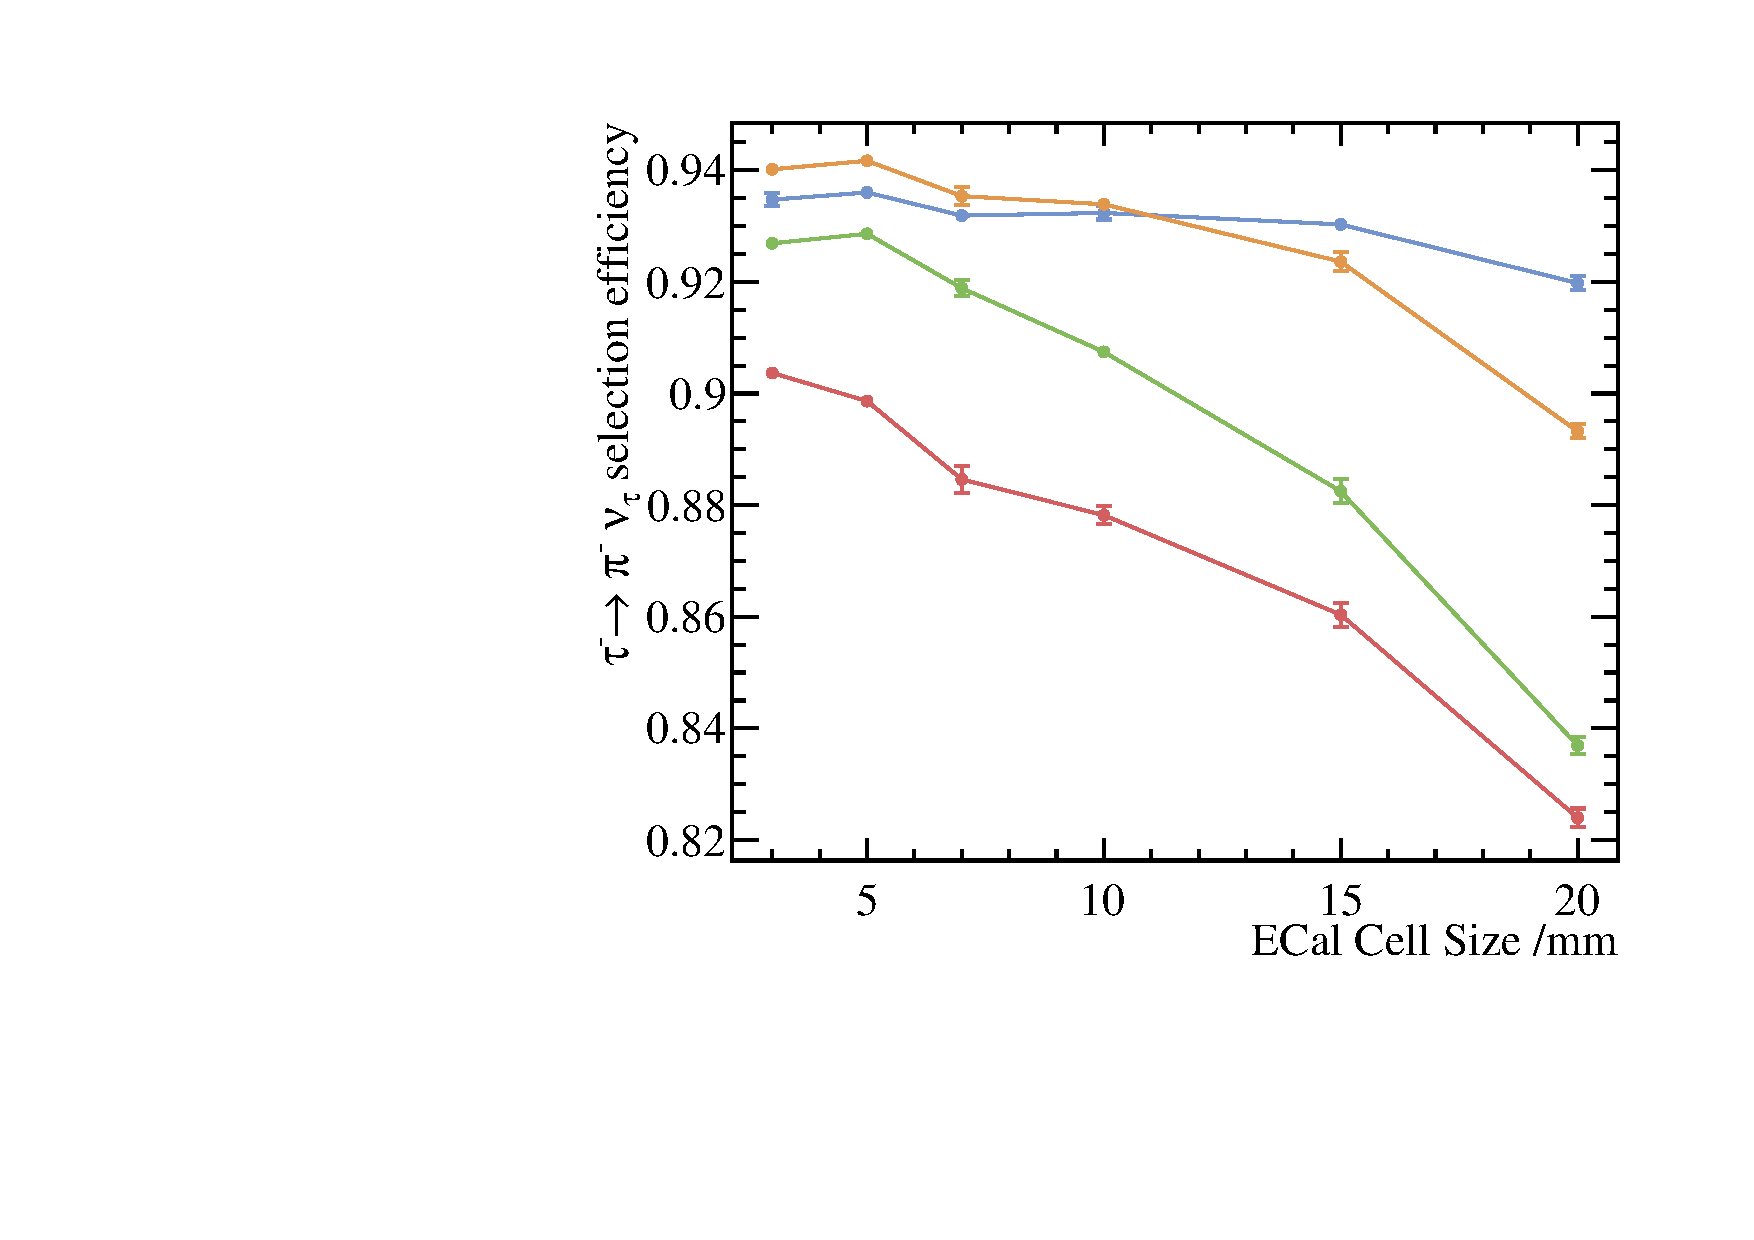
\includegraphics[width=.4\textwidth]{plots/pionSel}
\qquad
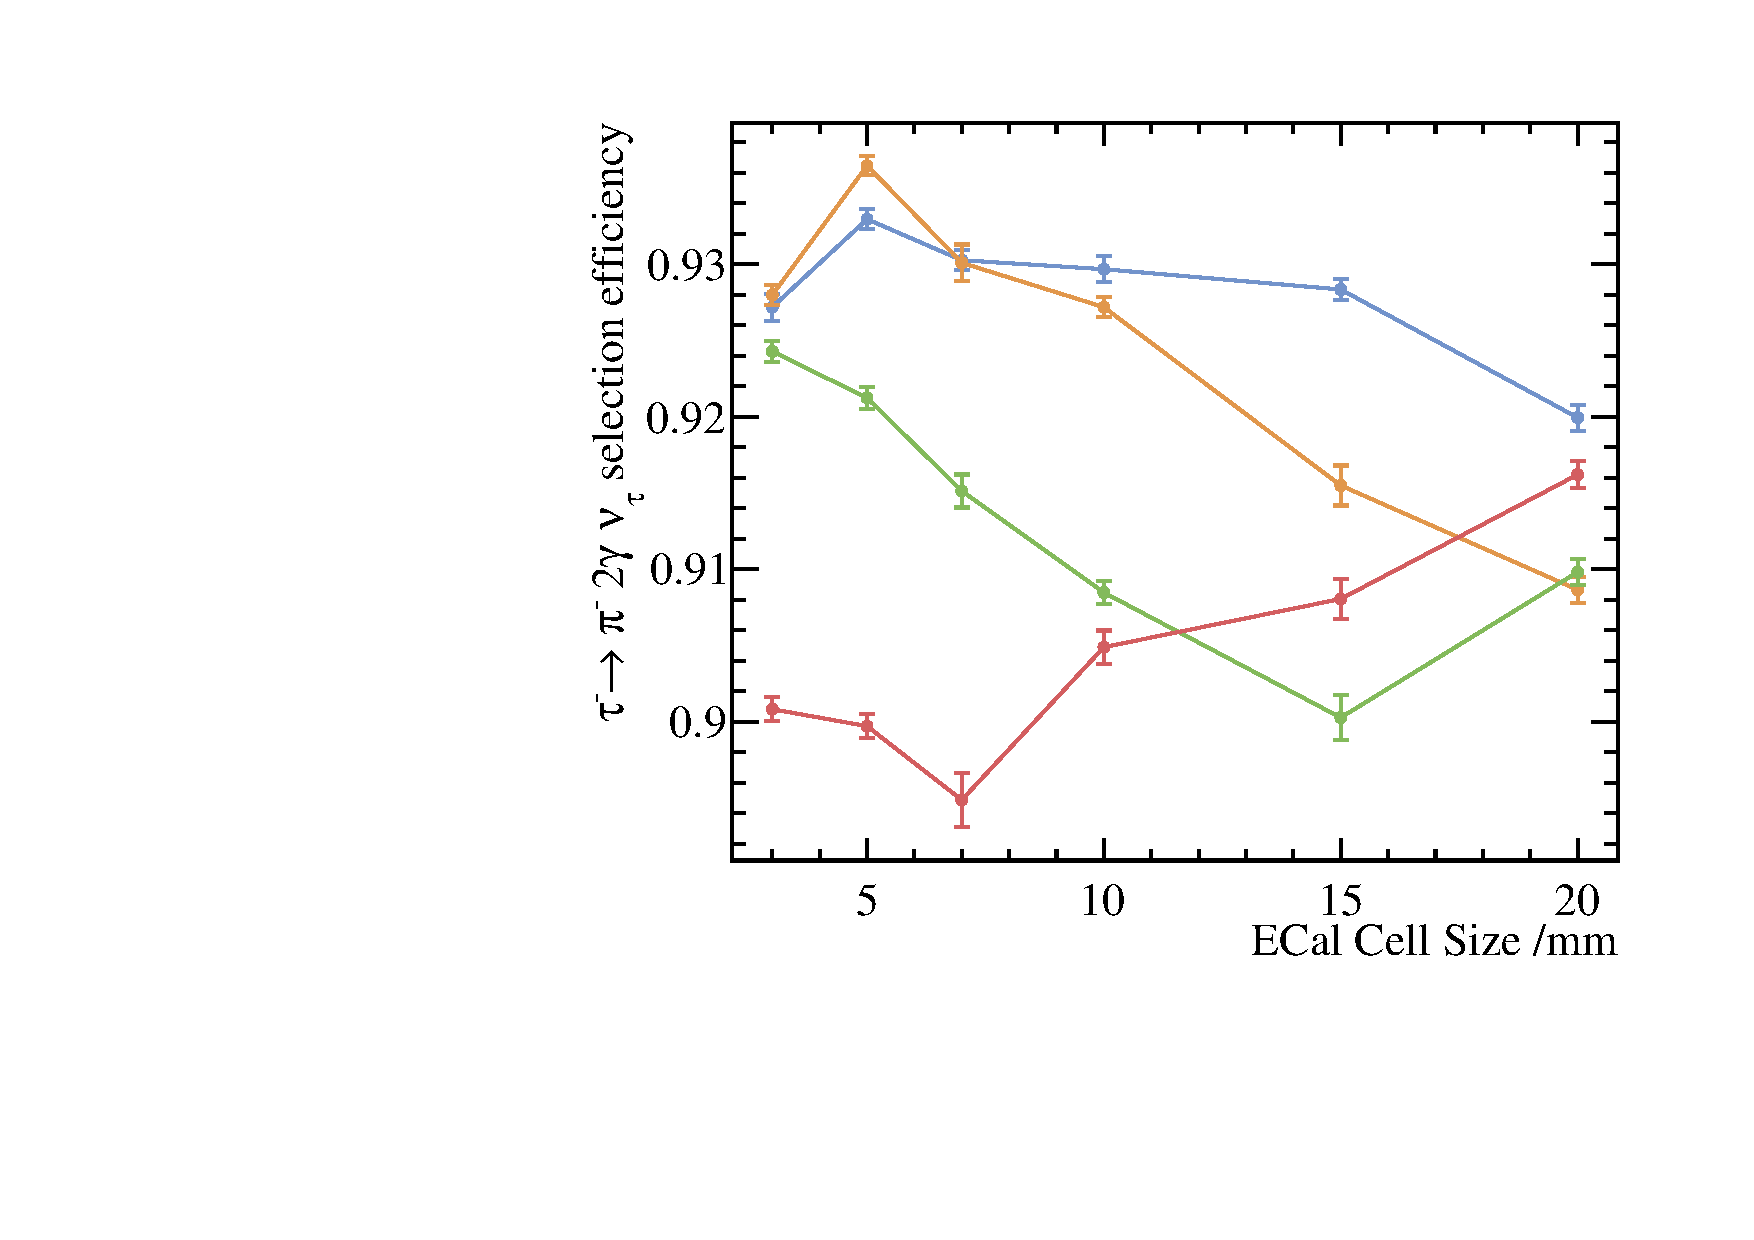
\includegraphics[width=.4\textwidth]{plots/pion2photon}
\qquad
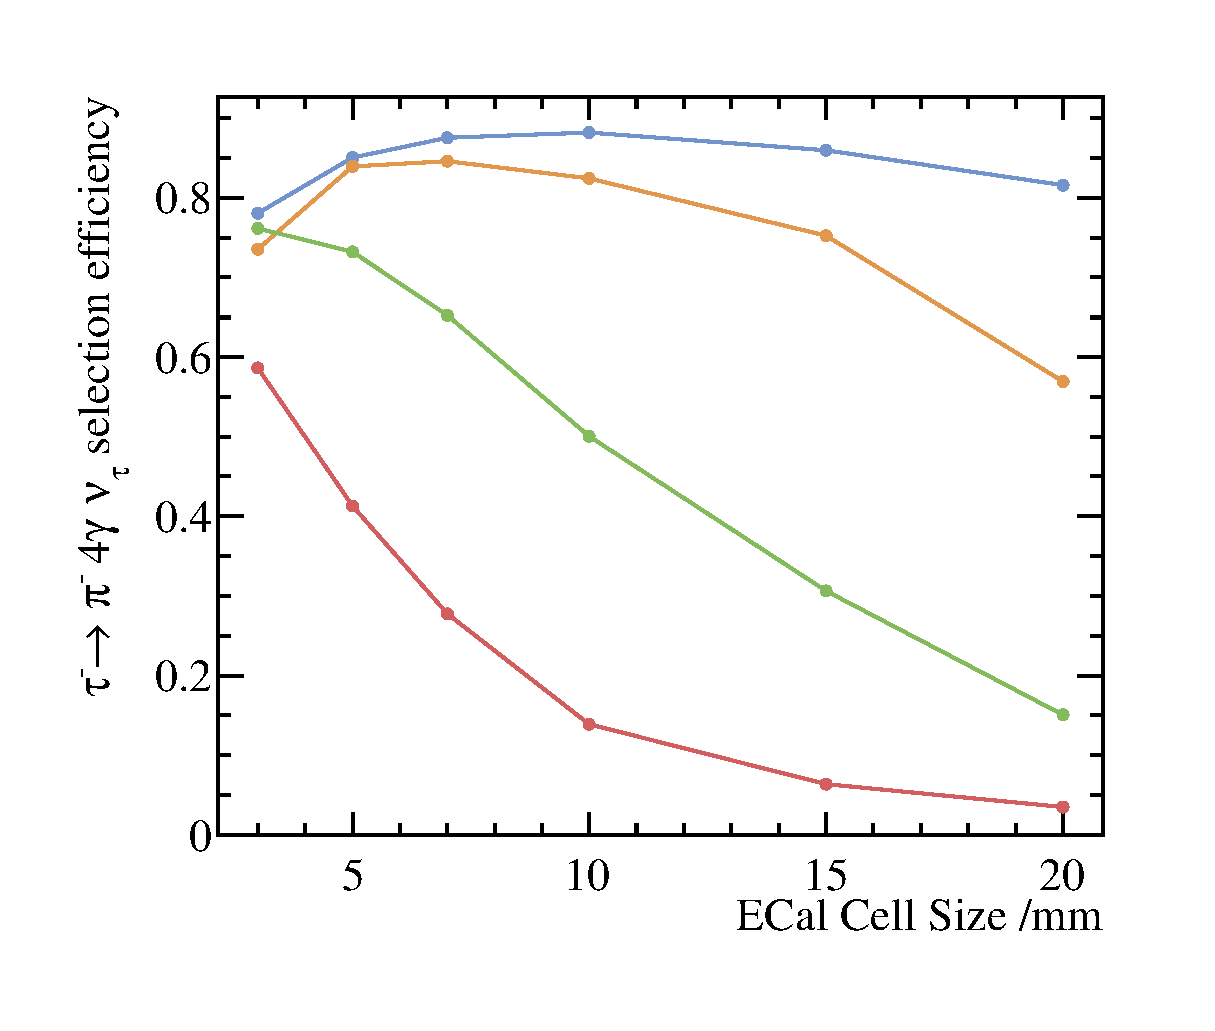
\includegraphics[width=.4\textwidth]{plots/pion4photon}
%\qquad
%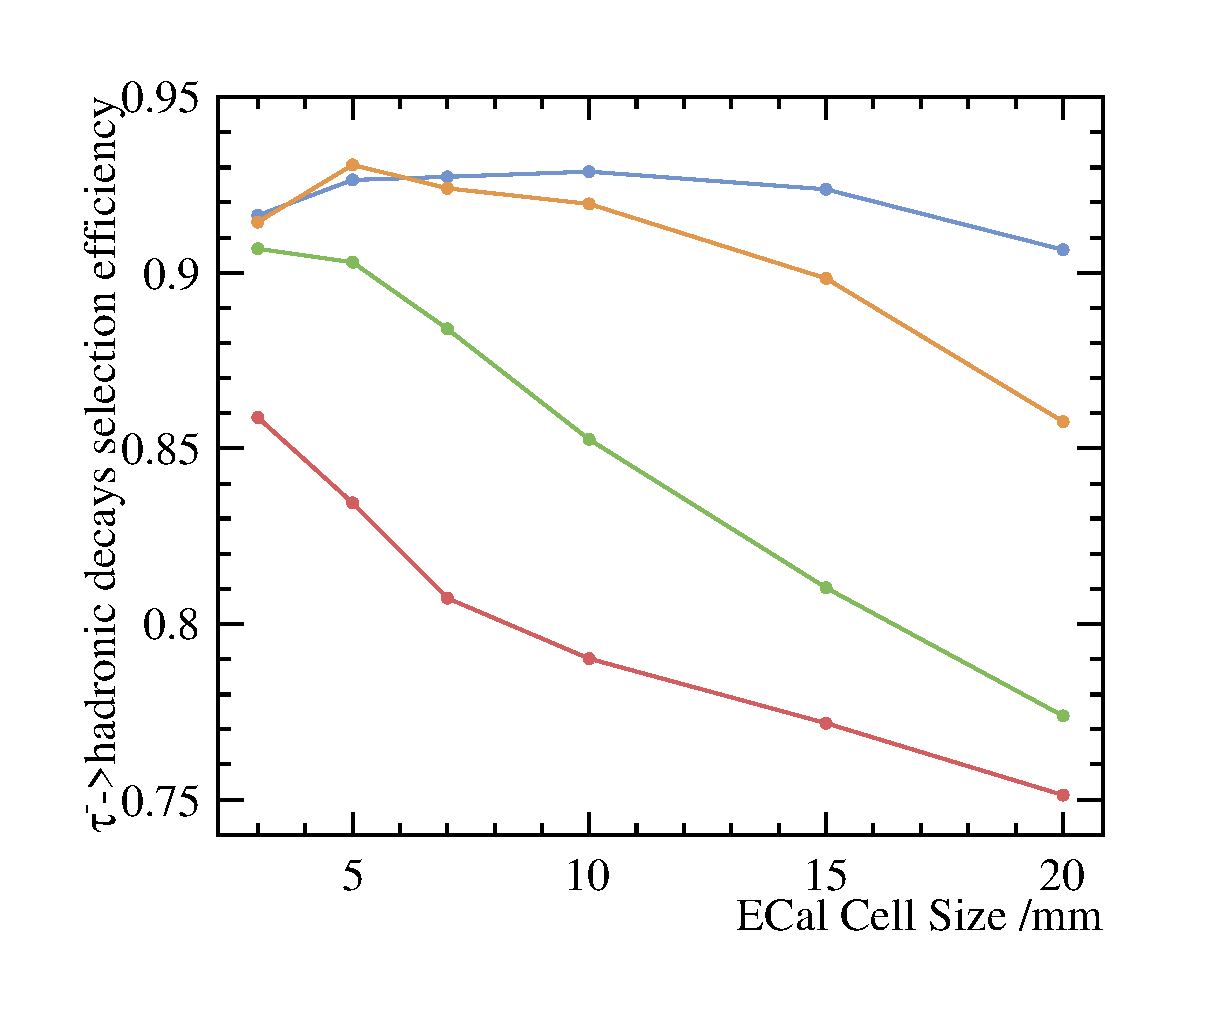
\includegraphics[width=.4\textwidth]{plots/hadEff}
% "\includegraphics" from the "graphicx" permits to crop (trim+clip)
% and rotate (angle) and image (and much more)
\caption{\label{fig:pion_efficiency} The selection efficiencies for various final states against the ECal cell size for different c.o.m. energies with the nominal CLIC\_ILD detector model are shown. The top left, top right and the bottom are for the \Ppiminus\Pnut, \Ppiminus2\Pphoton\Pnut and  \Ppiminus4\Pphoton\Pnut final states respectively. From the top to the bottom, blue, orange, green and red lines are representing the c.o.m. \Pelectron\APelectron collision energies of 100, 200, 500 and 1000\,GeV respectively.}
\end{figure}

To compare the impact of the ECAL cell sizes and the c.o.m. \Pelectron\APelectron collision energies on the separation of tau final states, the selection efficiencies for various final states against the ECal cell size for different c.o.m. energies are shown in the figure~\ref{fig:pion_efficiency}. 

Overall, the selection efficiency decreases as the c.o.m. energy increases. This is due to the fact that when {\Ptau}s are boosted at higher energies, the separation between decay products is smaller. Hence it is more difficult to reconstruct multi-photon final states correctly.

As the ECal cell sizes increase, the reconstruction efficiencies generally decrease. Larger cell sizes have lower spatial resolutions, making the separating of nearby photons more difficult.

For the \Ppiminus2\Pphoton\Pnut final state, the selection efficiency for 500\,GeV rises from ECal cell sizes 15\,mm to 20\,mm and the one for 1000\,GeV rises from 7\,, to 20\,mm actually goes up as cell size increases. This is because when the algorithm can not reconstruct \Ppiminus4\Pphoton\Pnut final state, the 4\Pphoton are often merged and the event topology would be very similar to the \Ppiminus2\Pphoton\Pnut final states. Hence more reconstructed events are identified as the \Ppiminus2\Pphoton\Pnut final state.

For the c.o.m. energy of 100 and 200\,GeV, the selection efficiency of the 5\,mm ECal cell size is better than that of the 3\,mm. One possible explanation is that the  and the PandoraPFA have been optimised for the nominal ILD detector with the 5\,mm ECal cell size, which shares the same ECal structure with the nominal CLIC\_ILD detector.

\begin{figure}[htbp]
\centering % \begin{center}/\end{center} takes some additional vertical space
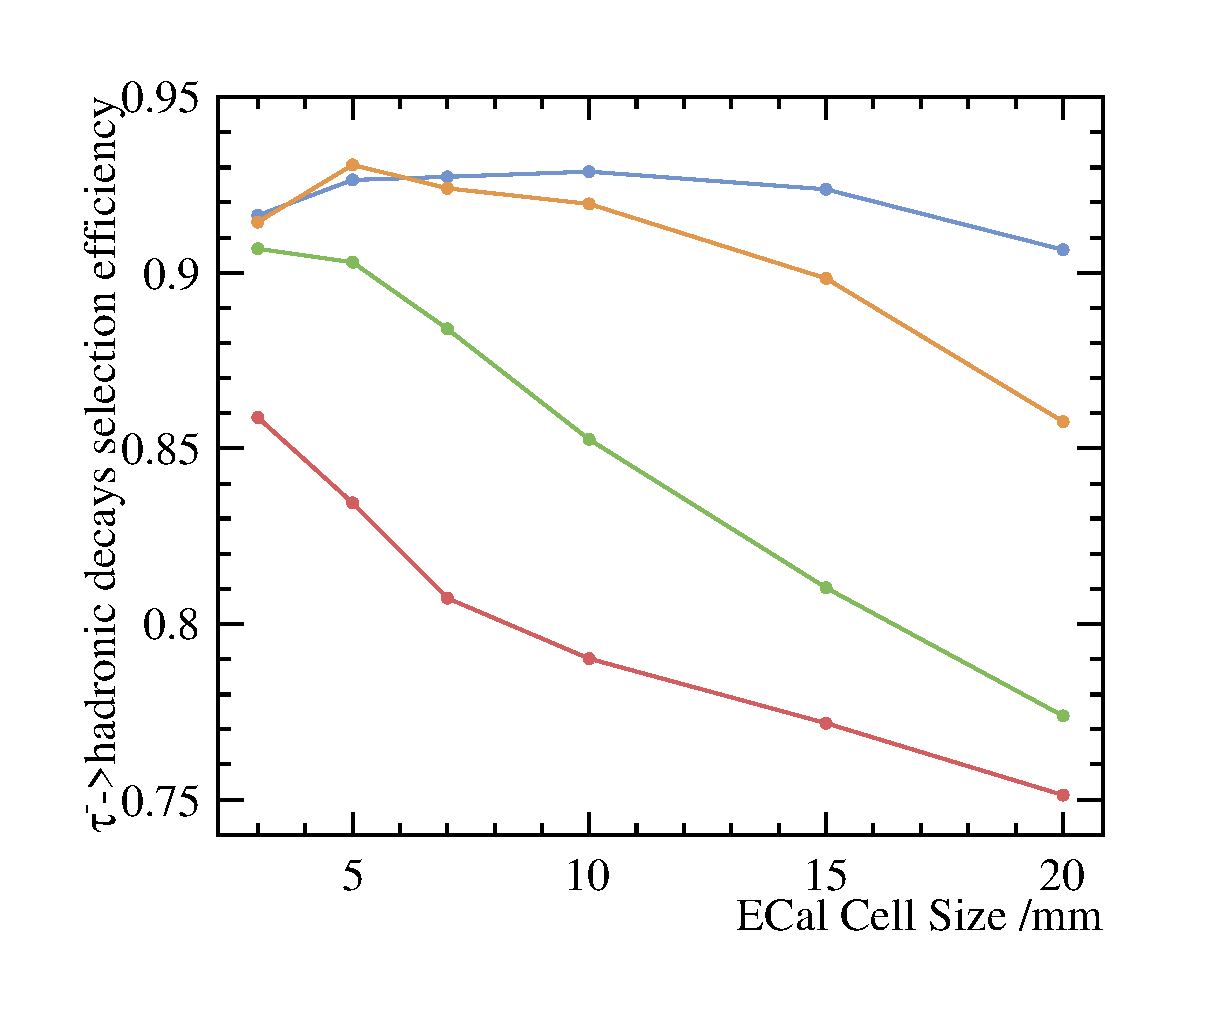
\includegraphics[width=.4\textwidth]{plots/hadEff}
% "\includegraphics" from the "graphicx" permits to crop (trim+clip)
% and rotate (angle) and image (and much more)
\caption{\label{fig:hadronic_efficiency} The \Ptau hadronic decay selection efficiency against the ECal cell size for different c.o.m. energies with the nominal CLIC\_ILD detector model are shown. The blue, orange, green and red lines are representing the c.o.m. \Pelectron\APelectron collision energies of 100, 200, 500 and 1000\,GeV respectively.}
\end{figure}

In order to compare the overall separation power of all the final states across c.o.m. energy and the ECal cell sizes, we constructed a single parameter function, the  \Ptau hadronic decay final state efficiency function, $\varepsilon_{hadronic} = \Sigma_{i} {Br}_{i}\varepsilon_{i} / \Sigma_{i} {Br}_{i}$, where $Br_{i}$ is the branching fraction of a final state after the generator level cut, $\varepsilon_{i}$ is the selection efficiency of the final state and the $i$ is summing over five hadronic decay final state of \Ptau. Leptonic decays, \Pelectron and \Pmuon, were not included as the variation of the leptonic decay selection efficiency is small.

In the figure~\ref{fig:hadronic_efficiency}, \Ptau hadronic decay final state efficiency, $\varepsilon_{hadronic}$, against the ECal cell size with different c.o.m. energy is shown. $\varepsilon_{hadronic}$ decreases when cell sizes increases and when c.o.m. increase.  Again, $\varepsilon_{hadronic}$ of the 5\,mm ECal cell size is better than that of the 3\,mm for 100 and 200\,GeV lines due the optimisation of the software fro the nominal ILD 5\,mm cell size.

The $\varepsilon_{hadronic}$ is above 90\% for the ECal cell size from 3 to 20\,mm for the c.o.m. energy of 100\,GeV. For 200\,GeV, the $\varepsilon_{hadronic}$ decreases from over 90\% to 86\% for the ECal cell size from 3 to 20\,mm. The degradation of the $\varepsilon_{hadronic}$ is significant for the 500 and 1000\,GeV lines, where the $\varepsilon_{hadronic}$ drops from over 90\% to 77\%  and from 86\% to 75\% respectively. 

%The degradation of $\varepsilon_{hadronic}$ is more significant for higher c.o.m. energy.

The paper illustrated the usage of reconstruction of the tau decay modes as a benchmark for the detector optimisation. 

%The high probability of correctly identifying the decay modes also showed the potential to measure the spin of the {\Ptau} with the CLIC machine.


%We discourage the use of inline figures (wrapfigure), as they may be
%difficult to position if the page layout changes.

%We suggest not to abbreviate: ``section'', ``appendix'', ``figure''
%and ``table'', but ``eq.'' and ``ref.'' are welcome. Also, please do
%not use \texttt{\textbackslash emph} or \texttt{\textbackslash it} for
%latin abbreviaitons: i.e., et al., e.g., vs., etc.



%\section{Sections}
%\subsection{And subsequent}
%\subsubsection{Sub-sections}
%\paragraph{Up to paragraphs.} We find that having more levels usually
%reduces the clarity of the article. Also, we strongly discourage the
%use of non-numbered sections (e.g.~\texttt{\textbackslash
%  subsubsection*}).  Please also see the use of
%``\texttt{\textbackslash texorpdfstring\{\}\{\}}'' to avoid warnings
%from the hyperref package when you have math in the section titles



%\appendix
%\section{Some title}
%Please always give a title also for appendices.


\acknowledgments

The authors would like thank P. G. Roloff for helping generating the simulated samples. 

%\paragraph{Note added.} This is also a good position for notes added
%after the paper has been written.





% We suggest to always provide author, title and journal data:
% in short all the informations that clearly identify a document.

\bibliographystyle{h-physrev3}
\bibliography{bib}

%\begin{thebibliography}{99}

%\bibitem{a}
%Author, \emph{Title}, \emph{J. Abbrev.} {\bf vol} (year) pg.

%\bibitem{b}
%Author, \emph{Title},
%arxiv:1234.5678.

%\bibitem{c}
%Author, \emph{Title},
%Publisher (year).


% Please avoid comments such as "For a review'', "For some examples",
% "and references therein" or move them in the text. In general,
% please leave only references in the bibliography and move all
% accessory text in footnotes.

% Also, please have only one work for each \bibitem.


%\end{thebibliography}
\end{document}
